
\setbeamertemplate{caption}{\raggedright\insertcaption\par}
\subsubsection{CAD input files}
\begin{frame}{CAD input files}

%Red faces (RGB=[255,0,0]): Fixture
%\item Green faces (RGB=[0,255,0]): Non-changing region  
%\item Colored (RGB=[0-255,0-255,0-255]): 3D loading vector 
%Linear force scaling: $F=f*({\bf x}-127)$\\
%One Byte: 0-126 negative, 127 zero, 128-255 positive direction
\begin{figure}
\centering
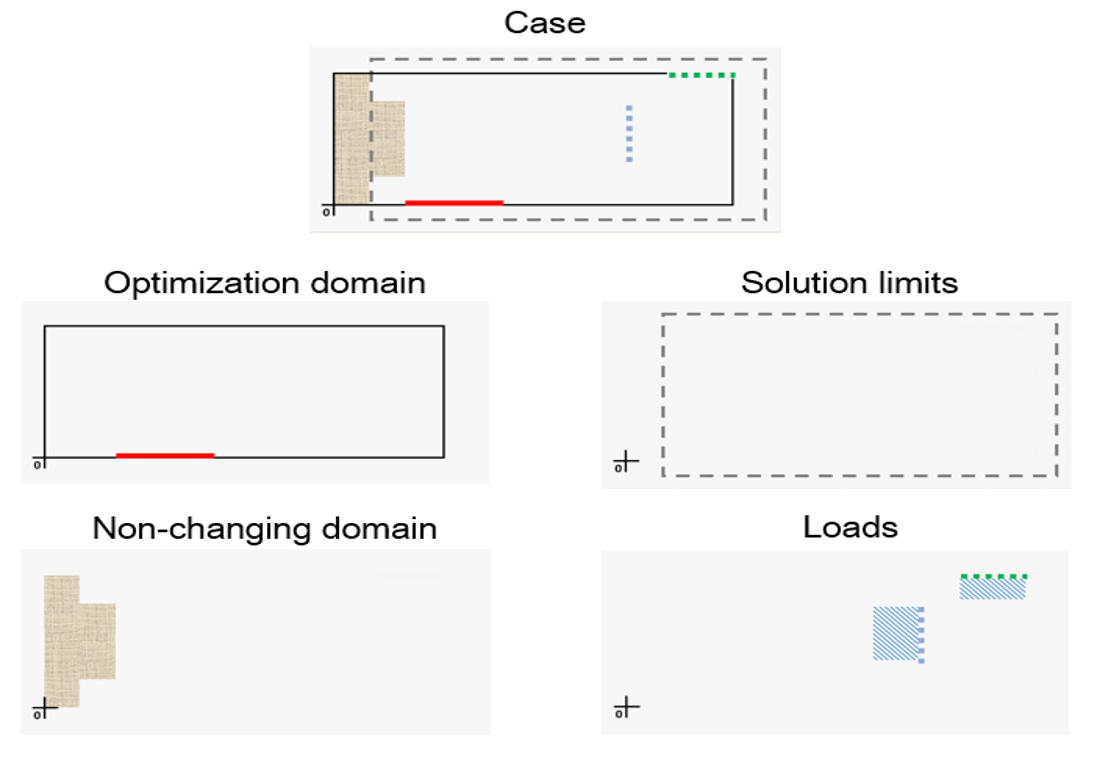
\includegraphics[width=.7\textwidth]{Pictures/SecondHalf/files_input.png}
\end{figure}
\end{frame}

\subsubsection{Voxelization}
\begin{frame}{Voxelized geometry}
\begin{itemize}
\item Done using OpenCascade  
\item Each region voxelized separately 
\end{itemize}
\vspace{0.4cm}
%\begin{enumerate}
%\item Active voxels (geometry)
%\item Fixture voxels
%\item Non-changing voxels
%\item Load voxels
%\end{enumerate}
\begin{minipage}{0.49\textwidth}
\begin{figure}
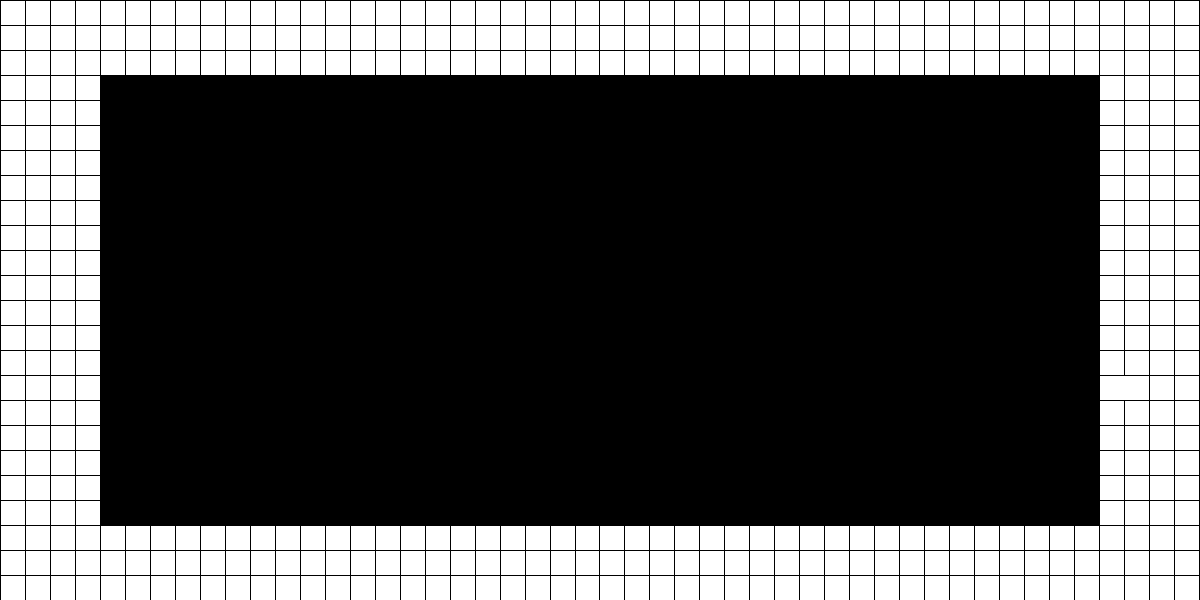
\includegraphics[width=.8\textwidth]{Pictures/Voxels/Active.pdf}
\caption{Participating voxels}
\end{figure}
\vspace{-0.6cm}
 \begin{figure}

\includegraphics[width=.8\textwidth]{Pictures/Voxels/NonChanging.pdf}
\caption{Non-Changing Voxels}
\end{figure}
\end{minipage}
\hfill
\begin{minipage}{0.49\textwidth}
\begin{figure}

\includegraphics[width=.8\textwidth]{Pictures/Voxels/Fixture.pdf}
\caption{Fixture voxels}
\end{figure}
\vspace{-0.6cm}
\begin{figure}

\includegraphics[width=.8\textwidth]{Pictures/Voxels/Load.pdf}
\caption{Load voxels}
\end{figure}
\end{minipage}
\end{frame}

\subsubsection{Black-Box Toplogy Optimizer}
\begin{frame}{Topology Optimization}
%Steps:
%\begin{enumerate}
%\item Geometry as voxel grid
%\item Calculate stress on geometry
%\item If stress in voxel below threshold %$\rightarrow$ remove voxel from active geometry
%\end{enumerate}
\only<1>{
\begin{figure}
\centering
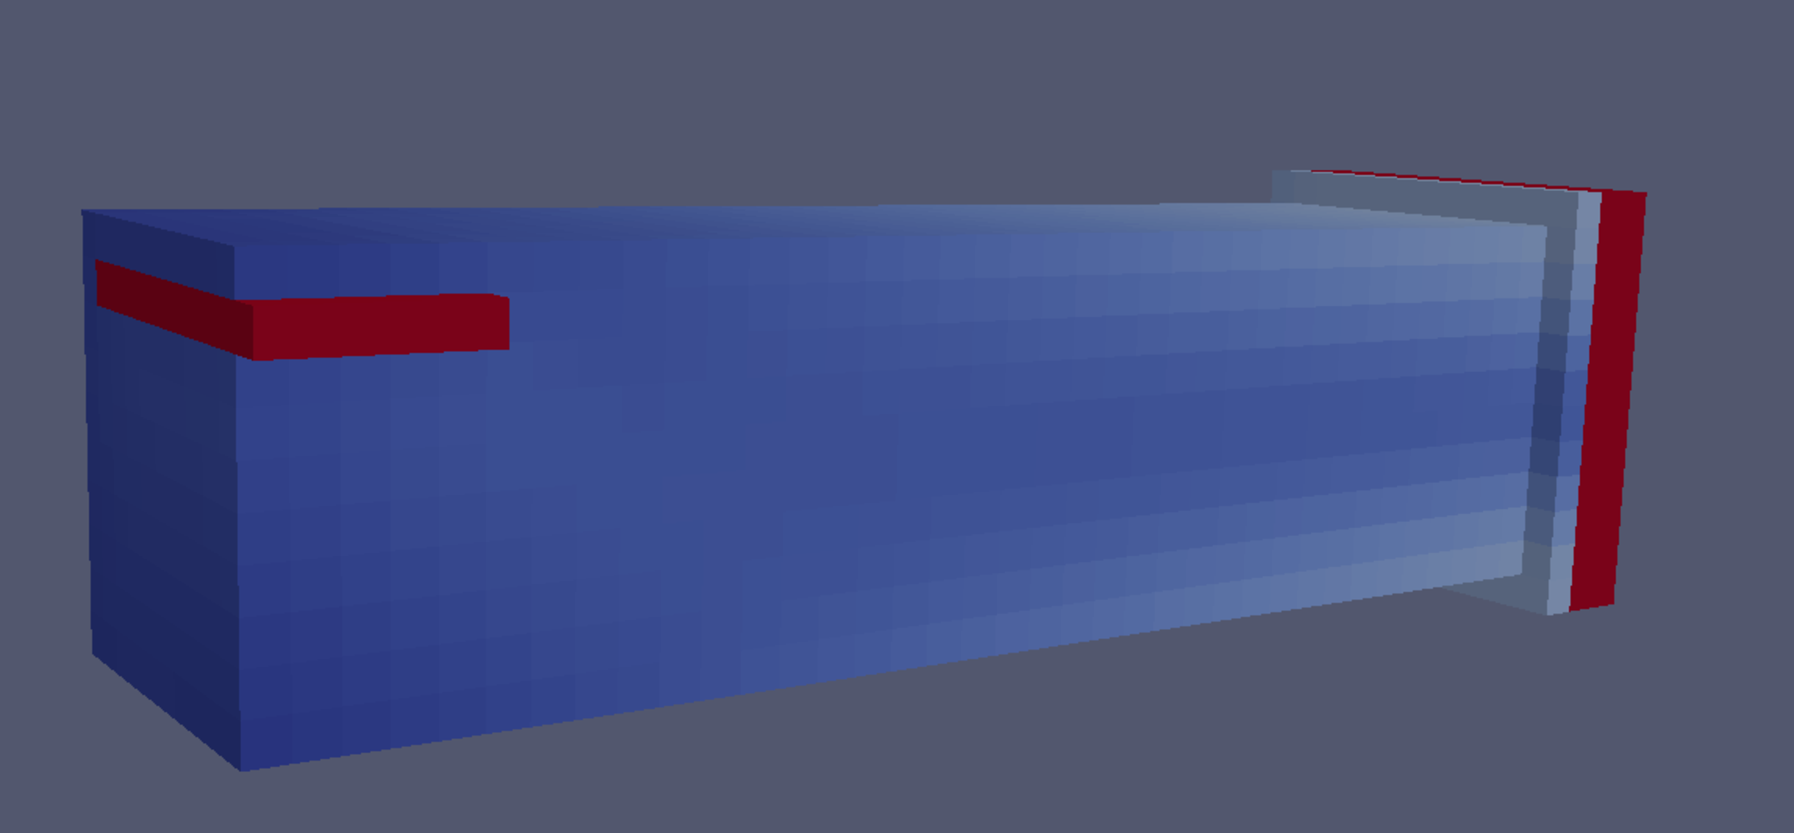
\includegraphics[width=.25\textwidth]{Pictures/TopOp/Cantilever_Topy_0.pdf}
\end{figure}}
\only<2>{
\begin{figure}
\centering
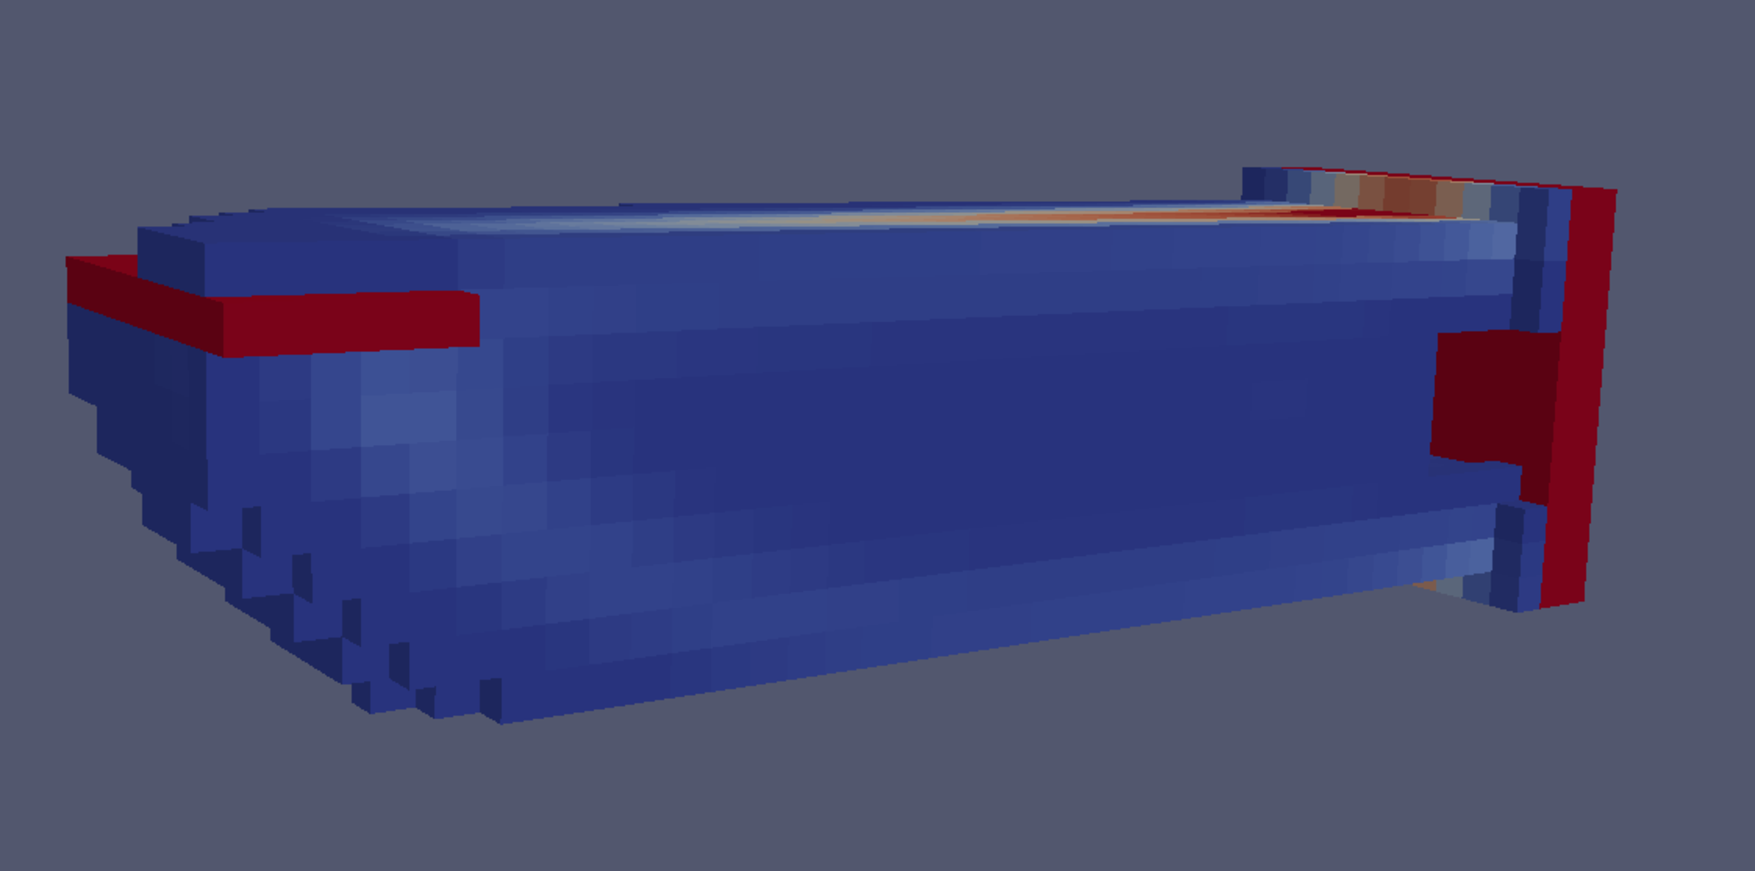
\includegraphics[width=.25\textwidth]{Pictures/TopOp/Cantilever_Topy_1.pdf}
\end{figure}}
\only<3>{
\begin{figure}
\centering
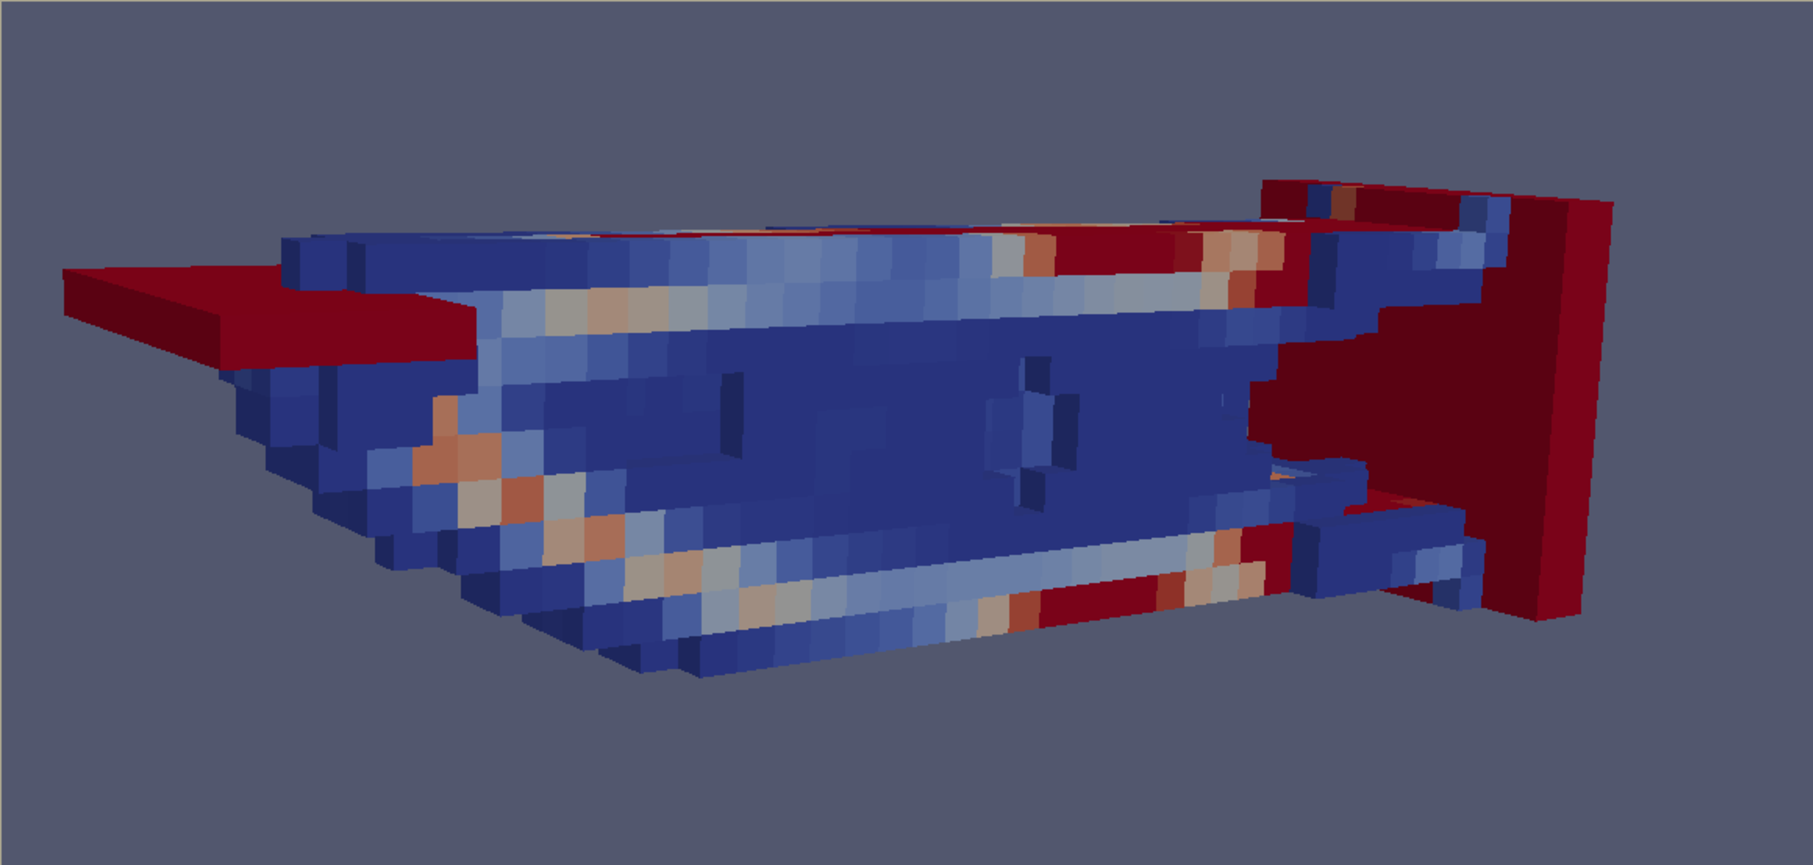
\includegraphics[width=.25\textwidth]{Pictures/TopOp/Cantilever_Topy_2.pdf}
\end{figure}}
\only<4>{
\begin{figure}
\centering
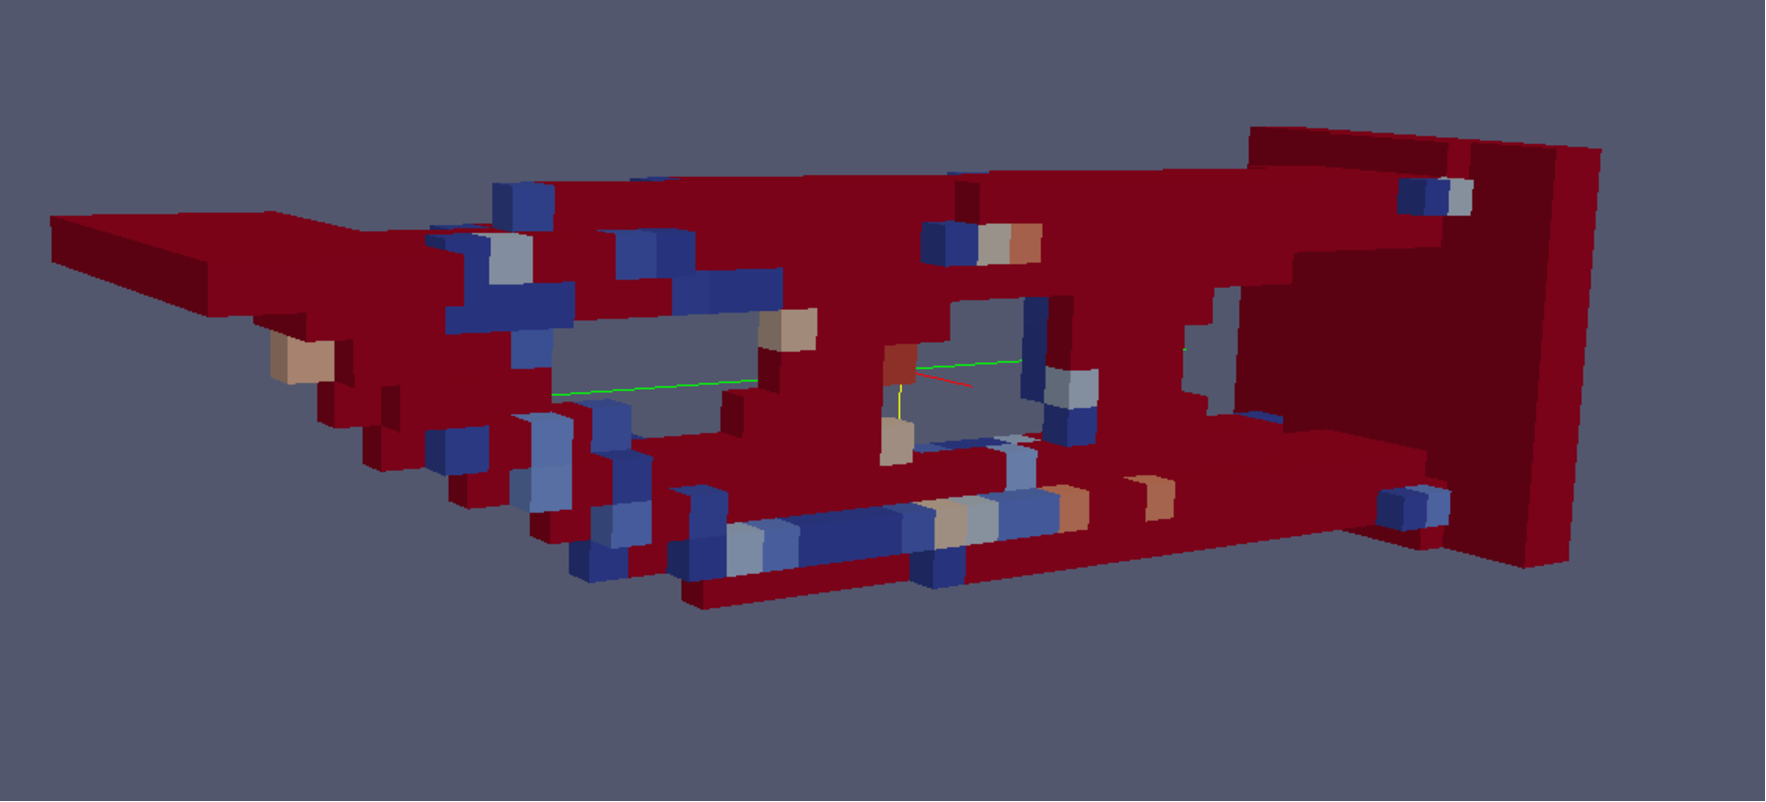
\includegraphics[width=.25\textwidth]{Pictures/TopOp/Cantilever_Topy_3.pdf}
\end{figure}}
\only<5>{
\begin{figure}
\centering
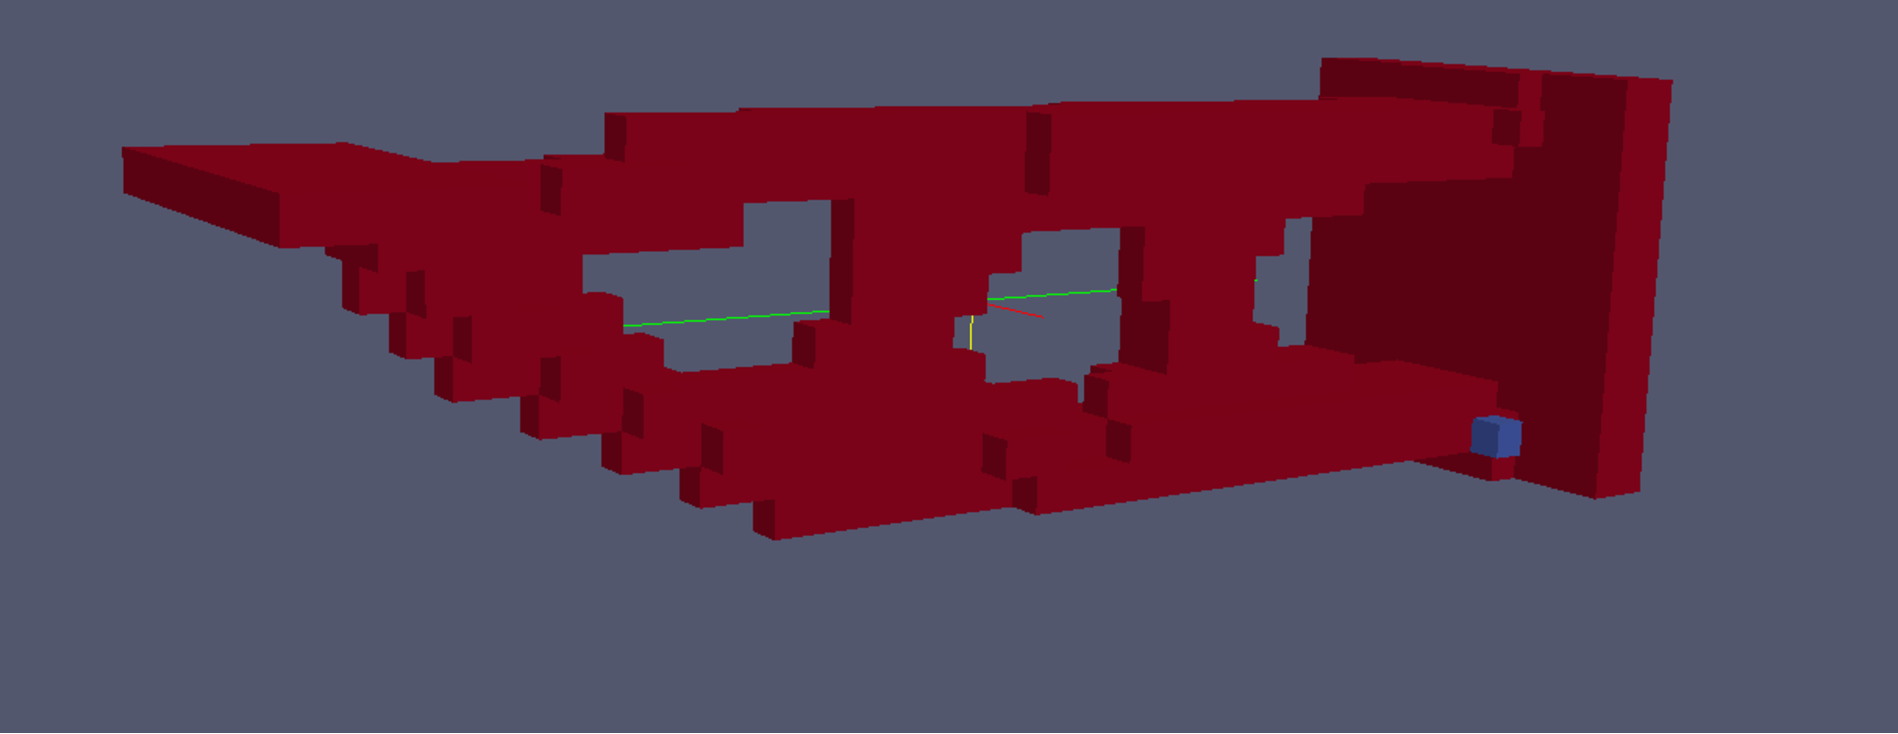
\includegraphics[width=.25\textwidth]{Pictures/TopOp/Cantilever_Topy_4.pdf}
\end{figure}}
\end{frame}
